\Chapter{Tervezés}

\section{A prototípusokról}
A fejlesztés során a prototípusokat használtam a funkciók önálló tesztelésére és a rendszer működésének ellenőrzésére. Mivel a fejlesztés felhasználói visszajelzés nélkül zajlott, a prototípusok iteratív elkészítése és folyamatos tesztelése segítette az alkalmazás stabilitásának és helyes működésének ellenőrzését. A különböző funkciók hozzáadása és tesztelése során minden egyes prototípus újabb funkciókkal bővült, majd ezek működését részletesen vizsgáltam, beleértve a konténerek kezelésének, a grafikus felület működésének, valamint a rendszererőforrás-mérő eszközök tesztelését is.

Tesztkódok vagy automatizált tesztelési eszközök használata helyett minden egyes funkciót manuálisan ellenőriztem, ami lehetővé tette a hibák gyors felismerését és azonnali javítását. Ez a folyamat különösen hasznos volt a terminál-emulátorral és a grafikus felülettel kapcsolatos interakciók esetében. Az egyes prototípusok közötti iterációk során így lépésről lépésre sikerült az alkalmazást stabil és használatra kész állapotba hozni.


\section{Az első Prototípus}

Az első prototípus célja egy alapvető grafikus felület létrehozása volt, amely lehetővé teszi a Docker konténerek egyszerű kezelését, monitorozását és naplózását, minimalizálva a parancssoros beavatkozások szükségességét. 

\begin{itemize}
	\item \textbf{Konténerek listázása és állapotkezelés:} A felhasználó számára lehetőséget biztosít a program, hogy az összes helyben futó Docker konténert listázza, azok állapotát megtekintse, és a kívánt konténereken gyorsan végezhesse az alapműveleteket, mint például az indítás, leállítás, eltávolítás.
	\item \textbf{Valós idejű erőforrás-monitorozás:} A program célja, hogy a futó konténerek CPU, memória és lemezhasználati adatainak megjelenítésével átlátható módon mutassa be az aktuális erőforrás-használatot, ezáltal segítve a felhasználót a teljesítményfigyelésben és az optimalizációban.
	\item \textbf{Konténerek naplóinak közvetlen elérése:} A Docker-naplók valós időben követhetők a terminálon keresztül, lehetőséget biztosítva a gyors hibakeresésre és diagnosztikára.
\end{itemize}

\subsection{Technológiai Megfontolások}
Az eszköz fejlesztéséhez a \textbf{Python} nyelvet és a \textbf{PyQt5} könyvtárat választottam, mivel ezek stabil és rugalmas fejlesztési környezetet biztosítanak a cross-platform GUI megvalósításához. A \textbf{Docker Python SDK} lehetővé teszi az egyszerű és gyors integrációt a Docker API-val, ami kulcsfontosságú volt a konténerkezelési funkciók implementációjához.

\begin{itemize}
	\item \textbf{Python és PyQt5:} A Python egyszerű szintaxisa és széles körű dokumentációja révén gyors fejlesztést és könnyű karbantarthatóságot biztosít, a PyQt5 könyvtár pedig átfogó eszközkészletet kínál az egyedi widgetek, gombok és grafikus elemek létrehozásához. Ennek segítségével könnyen kialakíthatóak a szükséges interakciók és vizuális komponensek.
	\item \textbf{Docker Python SDK:} Az SDK használatával könnyen végrehajthatóak a Docker API-n keresztüli alapvető műveletek, például konténerek listázása, indítása és leállítása. A fejlesztés során ez biztosította a szükséges funkcionális alapot, amelyre a GUI elemek ráépültek.
	\item \textbf{PyQtGraph a monitorozási funkciókhoz:} A PyQtGraph nagy teljesítményű grafikonokat és vizuális elemeket kínál, amelyeket a CPU, memória és diszkhasználat megjelenítésére használtam. Az adatok folyamatos frissítésével lehetőség van a konténerek valós idejű teljesítményének figyelésére, ami a felhasználók számára hasznos visszajelzést nyújt.
\end{itemize}

\subsection{Felhasználói Interfész Tervezése}
A felhasználói felület tervezése során fő szempont volt a kezelhetőség és az egyszerű, átlátható kialakítás, amely gyors hozzáférést biztosít az alapvető funkciókhoz.

\begin{itemize}
	\item \textbf{Konténerek listázása táblázatos formában:} A konténerek gombnyomásra egy táblázaton jelennek meg egy új ablakban. Az oszlopok az egyes konténerek alapadatait tartalmazzák, például az azonosítót, nevet és állapotot. Az egyes sorok mellett gombok találhatók a gyakran használt műveletekhez, mint a "Start", "Stop", "Remove".
	\item \textbf{Valós idejű monitorozási ablak:} Az erőforrás-használati grafikonokat különálló ablakban helyeztem el, amely CPU, memória és diszkhasználati adatokat tartalmaz. Az adatok folyamatos frissítésével biztosított, hogy a felhasználó azonnal lássa a konténer teljesítményváltozásait. Itt a tárhelyhasználat még nem valós adatokat jelenített meg.
	\item \textbf{Terminál ablak Docker-naplókhoz:} Az alkalmazás lehetőséget biztosít a konténernaplók valós idejű követésére egy külső terminál ablakban, amely automatikusan megnyílik a megfelelő konténer logjainak követéséhez.
\end{itemize}

\begin{figure}[H]
	\centering
	\begin{minipage}{0.45\textwidth}
		\centering
		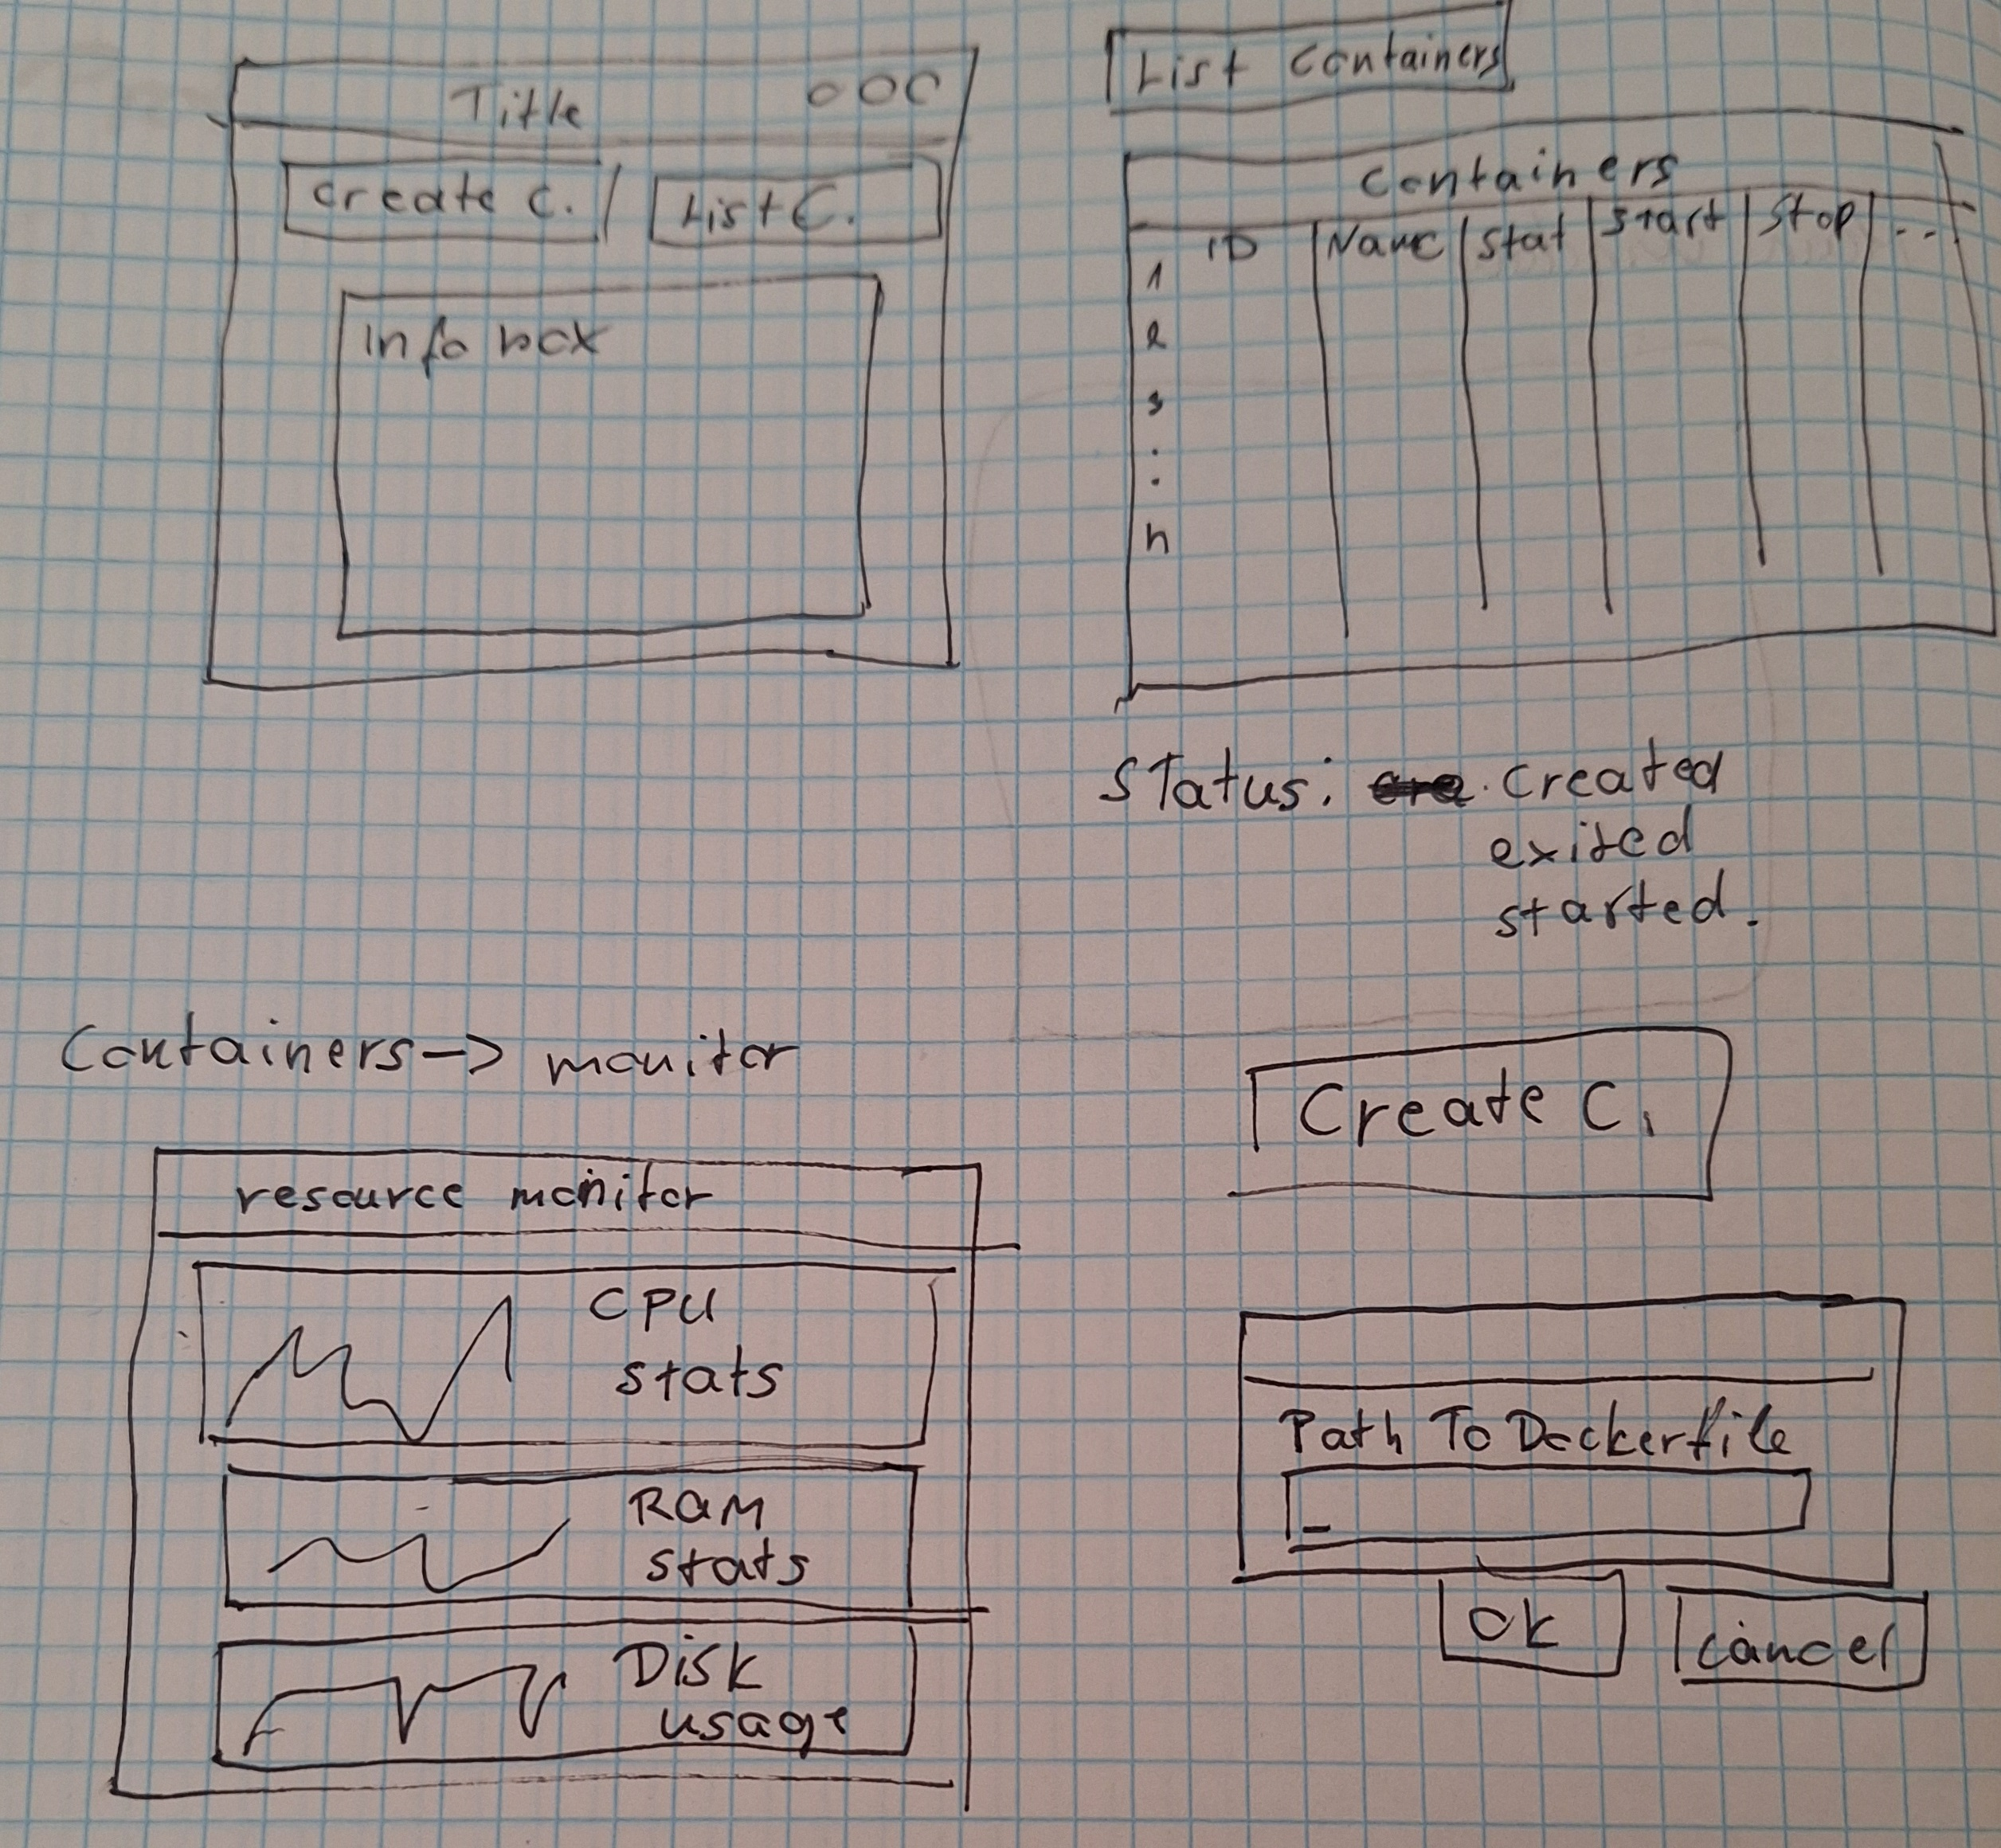
\includegraphics[width=1\linewidth]{images/first_design-draw}
		\caption{Az első tervrajz}
		\label{fig:firstdesign-draw}
	\end{minipage}
	\hfill
	\begin{minipage}{0.45\textwidth}
		\centering
		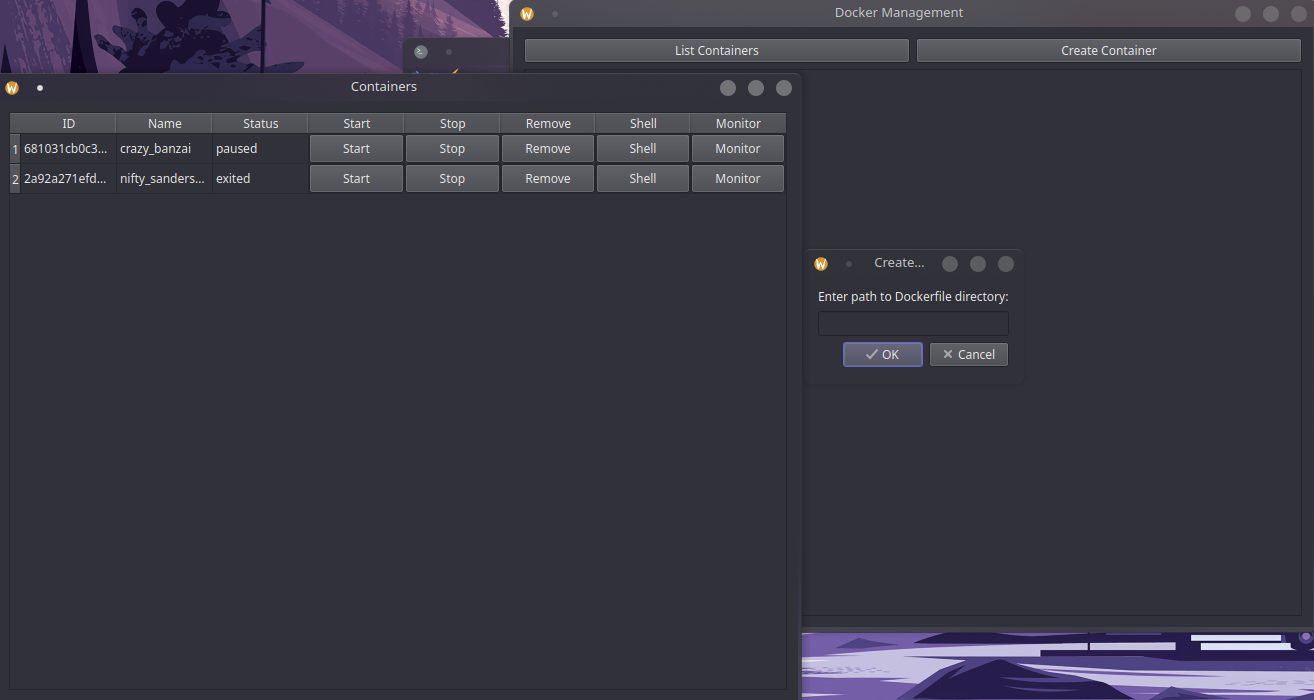
\includegraphics[width=1\linewidth]{images/0.0}
		\caption{Az elkészült prototípus}
		\label{fig:0}
	\end{minipage}
\end{figure}



\subsection{Első Prototípus Összegzése és Következő Lépések}
Az első prototípus segítségével sikerült egy stabil és alapvető Docker-kezelő eszközt létrehozni, amely lehetőséget ad az alapvető konténerműveletek gyors és intuitív végrehajtására. A tesztelés során nyert tapasztalatok alapján a következő fejlesztési irányokat határoztuk meg:

\begin{itemize}
	\item \textbf{Kibővített monitorozási lehetőségek:} A következő iterációkban a monitorozási funkciókat tovább bővítjük, hogy részletesebb és pontosabb teljesítményadatokat biztosítsanak.
	\item \textbf{Naplózási és hibakeresési funkciók javítása:} További fejlesztések szükségesek a naplózási és hibanaplózási funkciókban, így a felhasználók több részletes információhoz jutnak a konténerek viselkedéséről.
	\item \textbf{Felhasználói felület további finomítása:} A következő verziók során egyszerűbb és átláthatóbb kezelőfelületet kívánunk létrehozni, amely jobban illeszkedik a felhasználói igényekhez és könnyebbé teszi a navigációt.
	\item \textbf{Kód modularizálása:} A kód kezdetben egyetlen fájlban valósult meg, de a jövőben szükségessé válik a kód felosztása különálló modulokra. A külön fájlokba szervezett kód lehetővé teszi a könnyebb karbantartást és bővítést.
\end{itemize}

\newpage
\section{Továbbfejlesztett Prototípus: Docker GUI}

\subsection{Új Fejlesztések}

Az alkalmazásban számos új fejlesztést vezettem be az új verziókban a teljesítmény javítása érdekében.
Az egyik jelentős újítás a szálkezelés alkalmazása a Resource Monitor funkcióban. A hosszú ideig tartó erőforrás-monitorozási műveletek, mint például a CPU és memória használat követése, most már külön szálon futnak. Ez lehetővé teszi, több egyszerre futó konténer monitrozását. Ehhez a QThread osztályt alkalmaztam, amely lehetővé teszi az aszinkron működést. A szálkezelés segítségével a program képes kezelni a háttérben futó feladatokat anélkül, hogy az alkalmazás teljesítménye csökkenne.

A naplózási rendszer kifejlesztése is prioritás volt. Az alkalmazás mostantól kétféle naplózási szinttel működik. A hibák és figyelmeztetések naplózása mellett részletes információkat rögzítünk a program futásáról, amelyeket a felhasználók számára is elérhetővé teszünk a konzolon és egy log fájlban. Ezen kívül a hibák részletesebb információkat adnak a fellépő problémák okairól, így a felhasználók könnyebben diagnosztizálhatják és elháríthatják a hibákat.

A konténerműveletek kezelése is bővítésen esett át. Most már egyszerűbb módon érhetők el a legfontosabb műveletek, mint a konténerek indítása, leállítása, szüneteltetése és újraindítása. A különböző műveletekhez gombok és megfelelő kezelőfelület segíti a felhasználókat a gyors és egyszerű végrehajtásban. A konténerek állapotáról és egyéb jellemzőiről is részletesebb információk jelennek meg, amelyek segítik a felhasználókat abban, hogy pontosan lássák, mi történik a rendszerben.

A képek és hálózatok kezelése is kibővült. A program most már nemcsak a konténerek, hanem a Docker képek és hálózatok kezelésére is lehetőséget biztosít. A felhasználók könnyen listázhatják a képeket, törölhetik azokat, illetve új hálózatokat hozhatnak létre vagy távolíthatnak el. Az egyes műveletek gyors végrehajtását gombok segítik.

A felhasználói felület is finomításra került. Az új dizájn lehetővé teszi a gyorsabb navigációt, miközben egyszerűsíti a különböző funkciók elérését. Az új verzióban a gombok és táblázatok elrendezése átláthatóbbá vált, így a felhasználók könnyebben kezelhetik a Docker környezetüket.

A következő lépések során tovább javítjuk az alkalmazás stabilitását, és az új Docker verziókkal való kompatibilitást biztosítjuk. A jövőbeli fejlesztések között szerepel a Docker Compose fájlok kezelése, valamint a konténerek közötti interakciók egyszerűsítése is. Mindezek célja, hogy a rendszer még inkább felhasználóbarát és hatékony legyen.


\begin{figure}[H]
	\centering
	\begin{minipage}{0.45\textwidth}
		\centering
		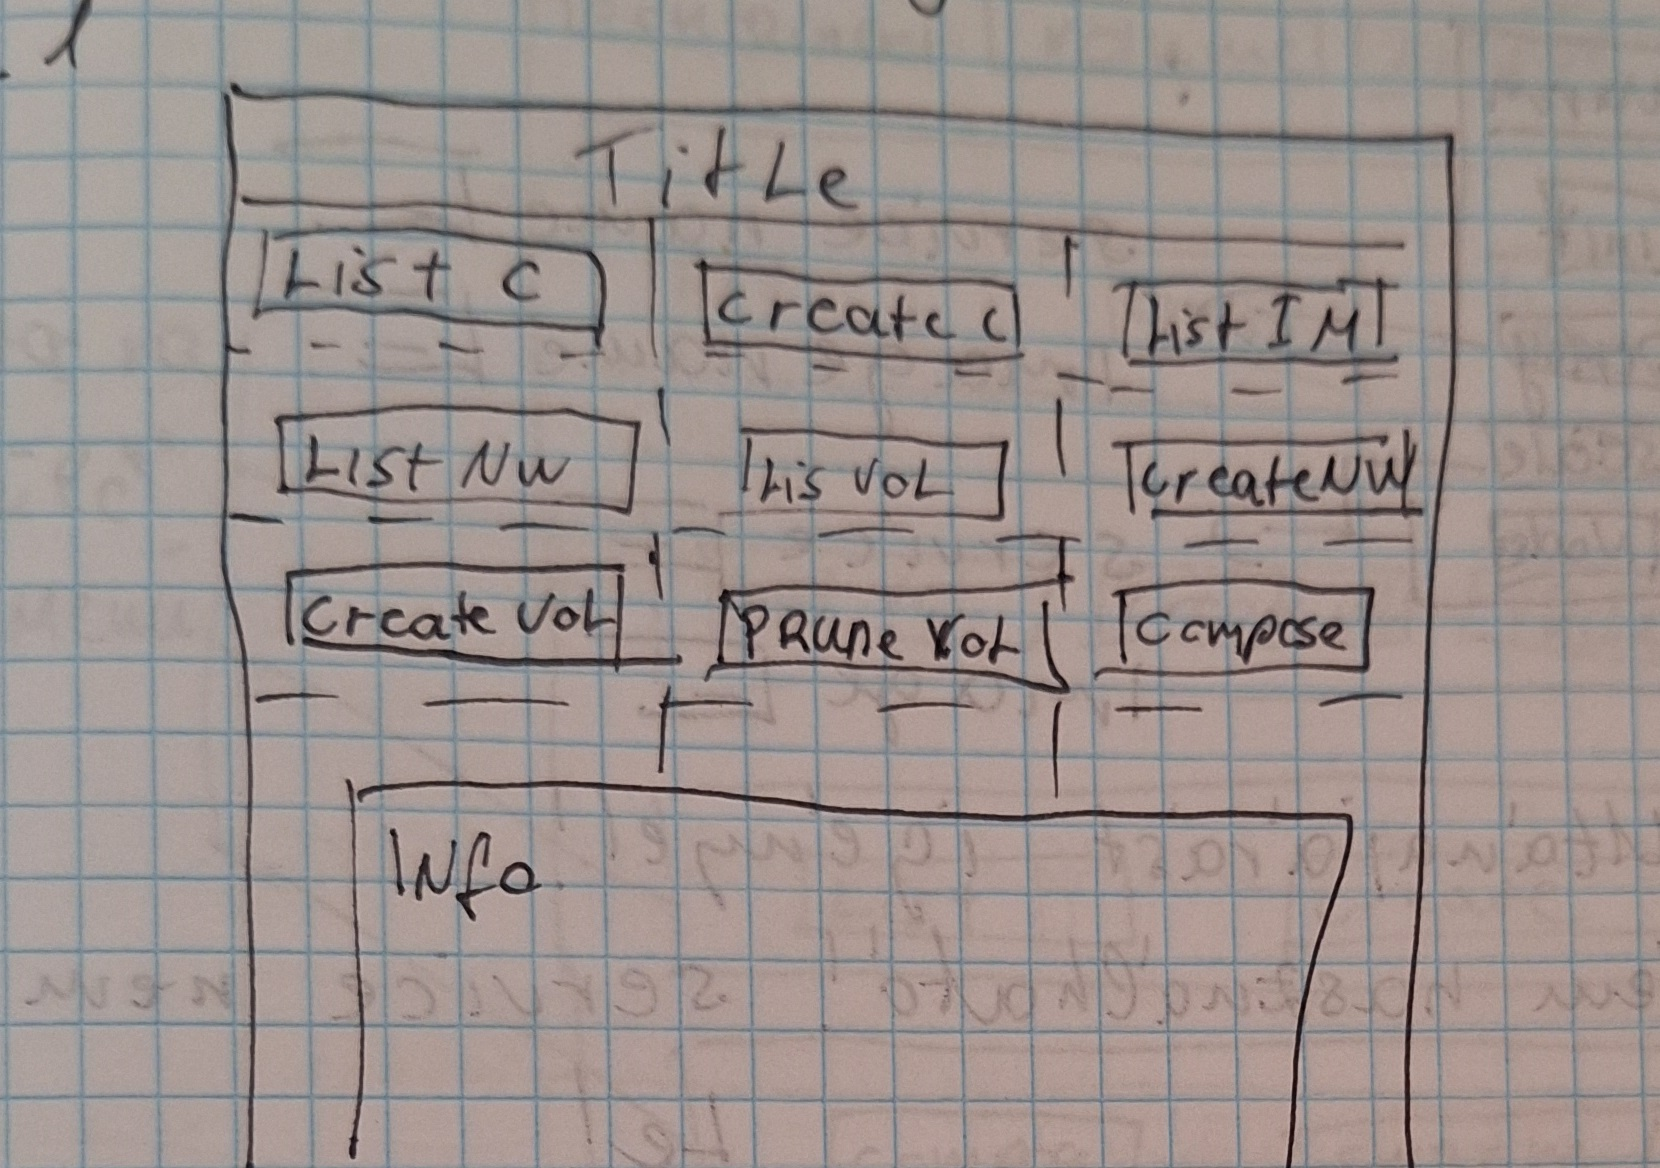
\includegraphics[width=1\linewidth]{images/2nd_design}
		\caption{A második tervrajz}
		\label{fig:2nd_design}
	\end{minipage}
	\hfill
	\begin{minipage}{0.45\textwidth}
		\centering
		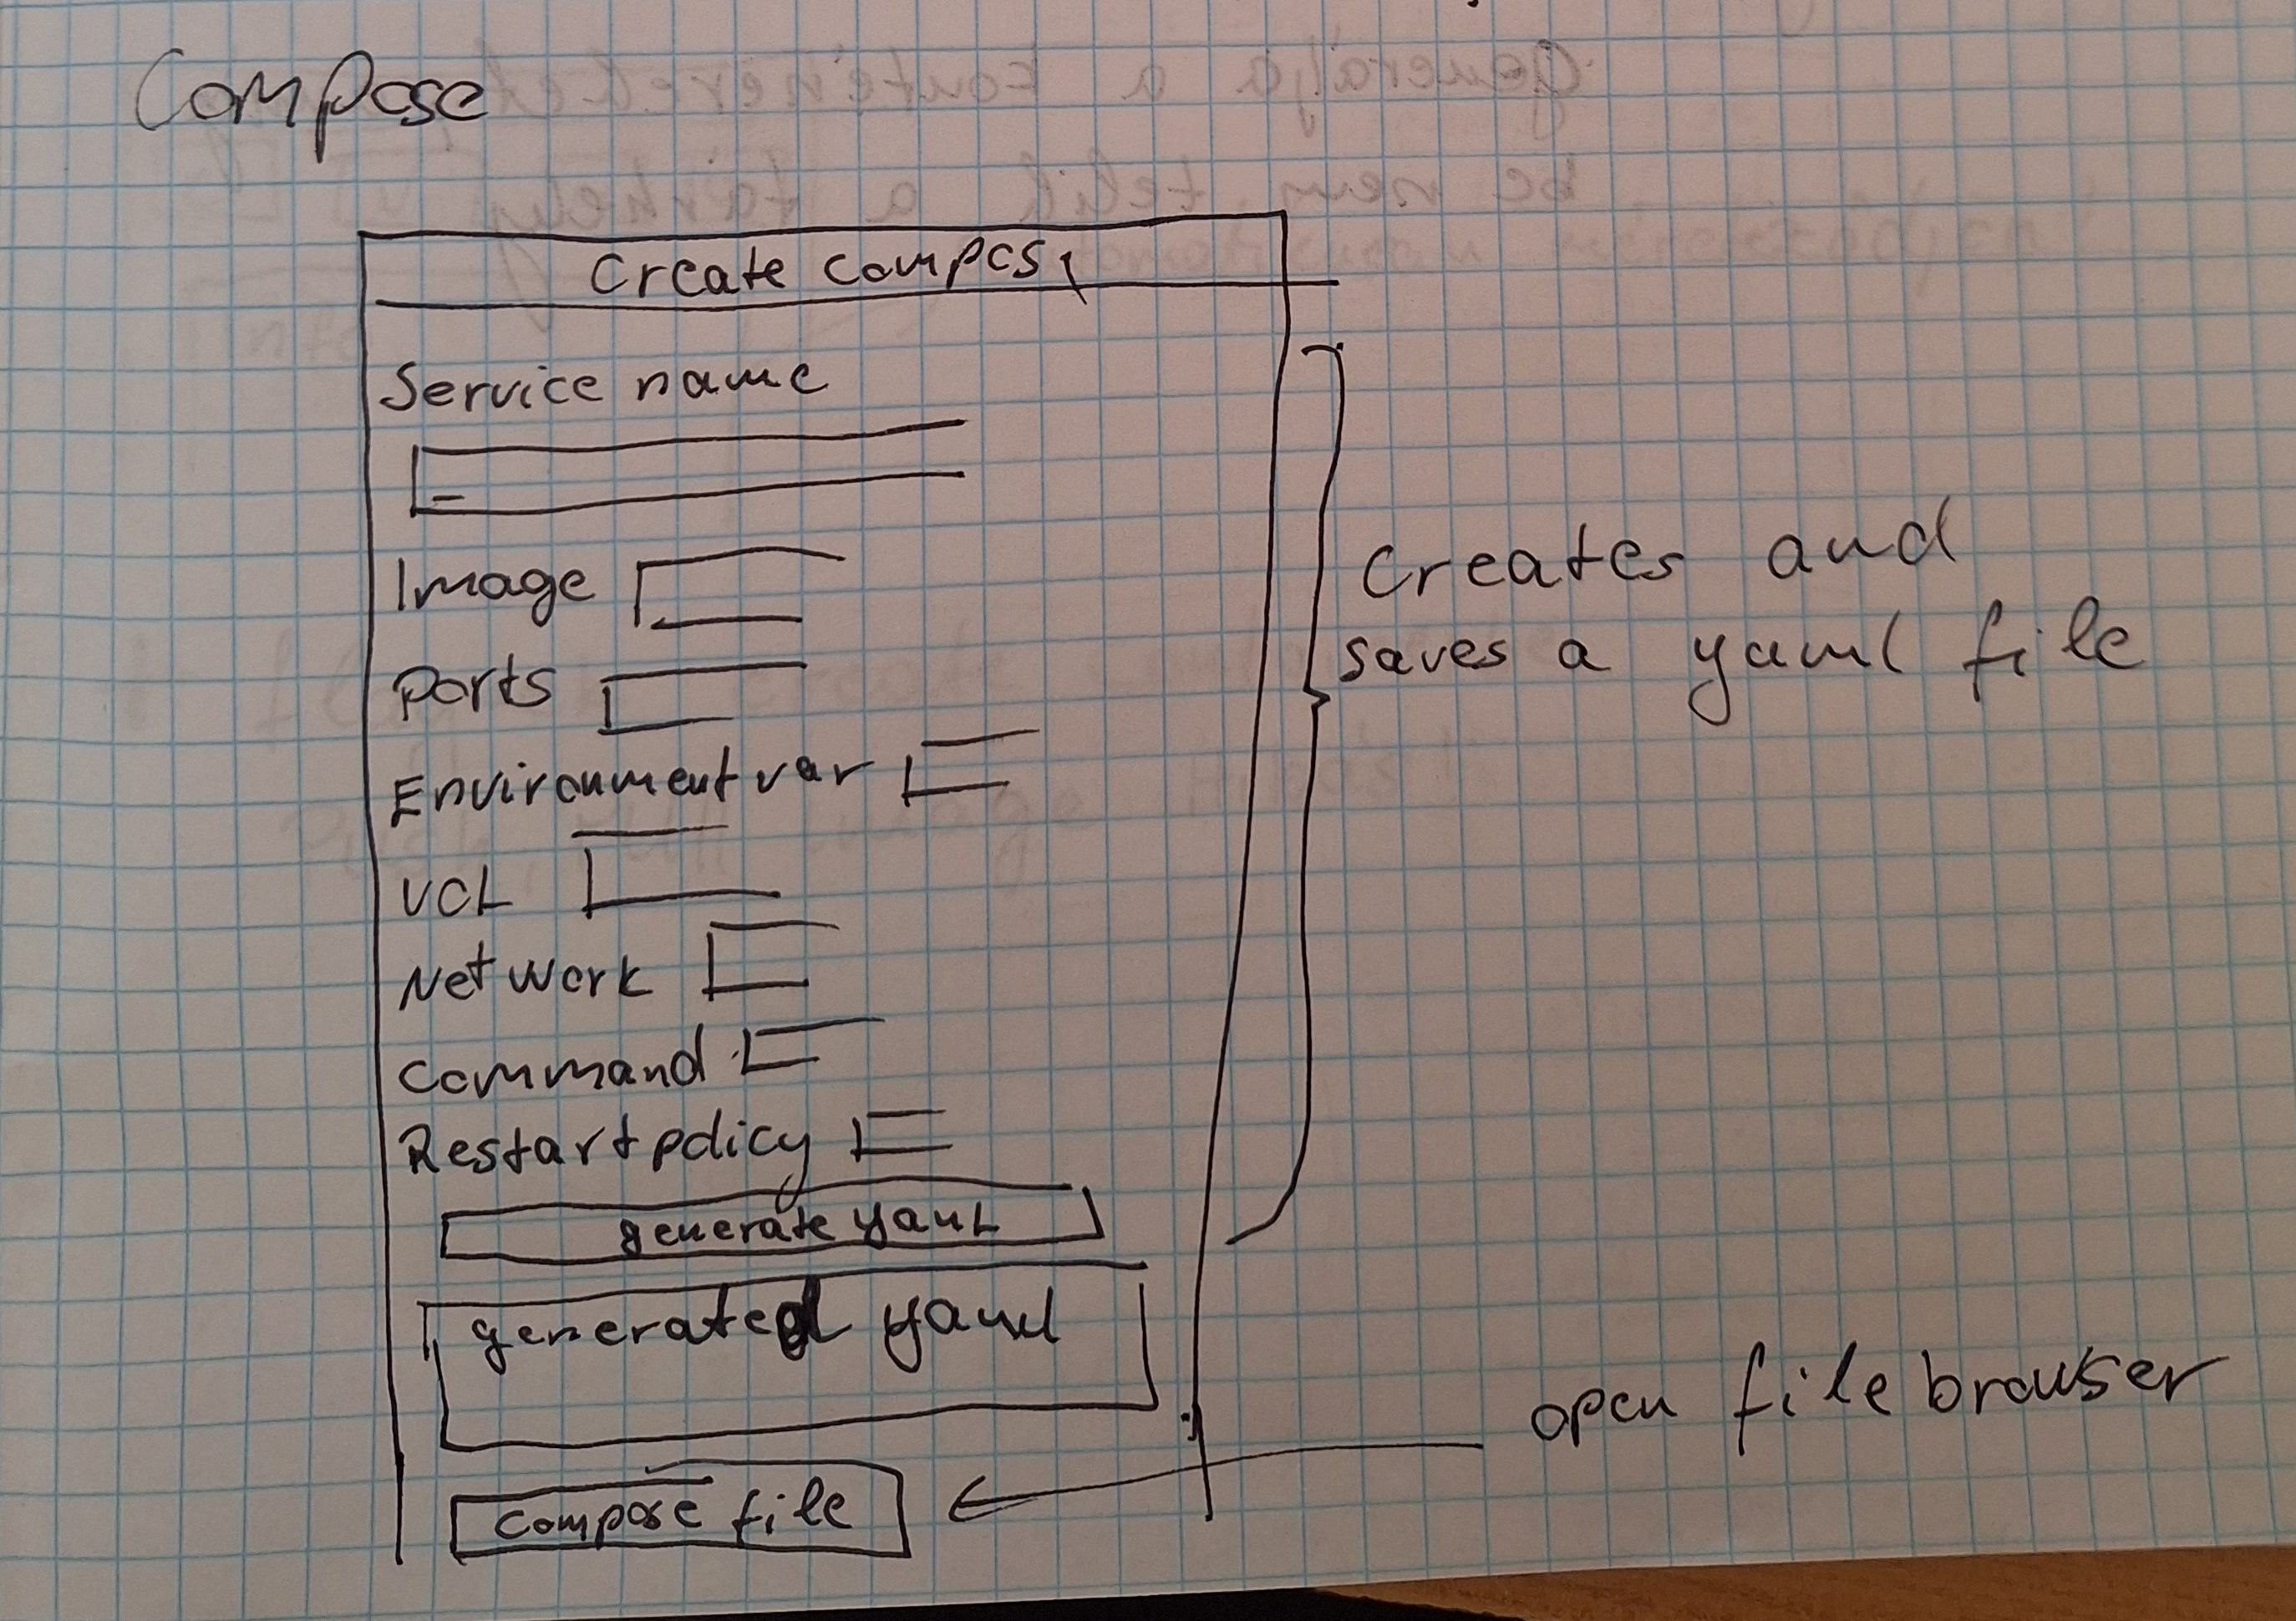
\includegraphics[width=1\linewidth]{images/1st_compose}
		\caption{Docker Compose kezelő felület}
		\label{fig:1st_compose}
	\end{minipage}
\end{figure}


\begin{figure}[H]
	\centering
	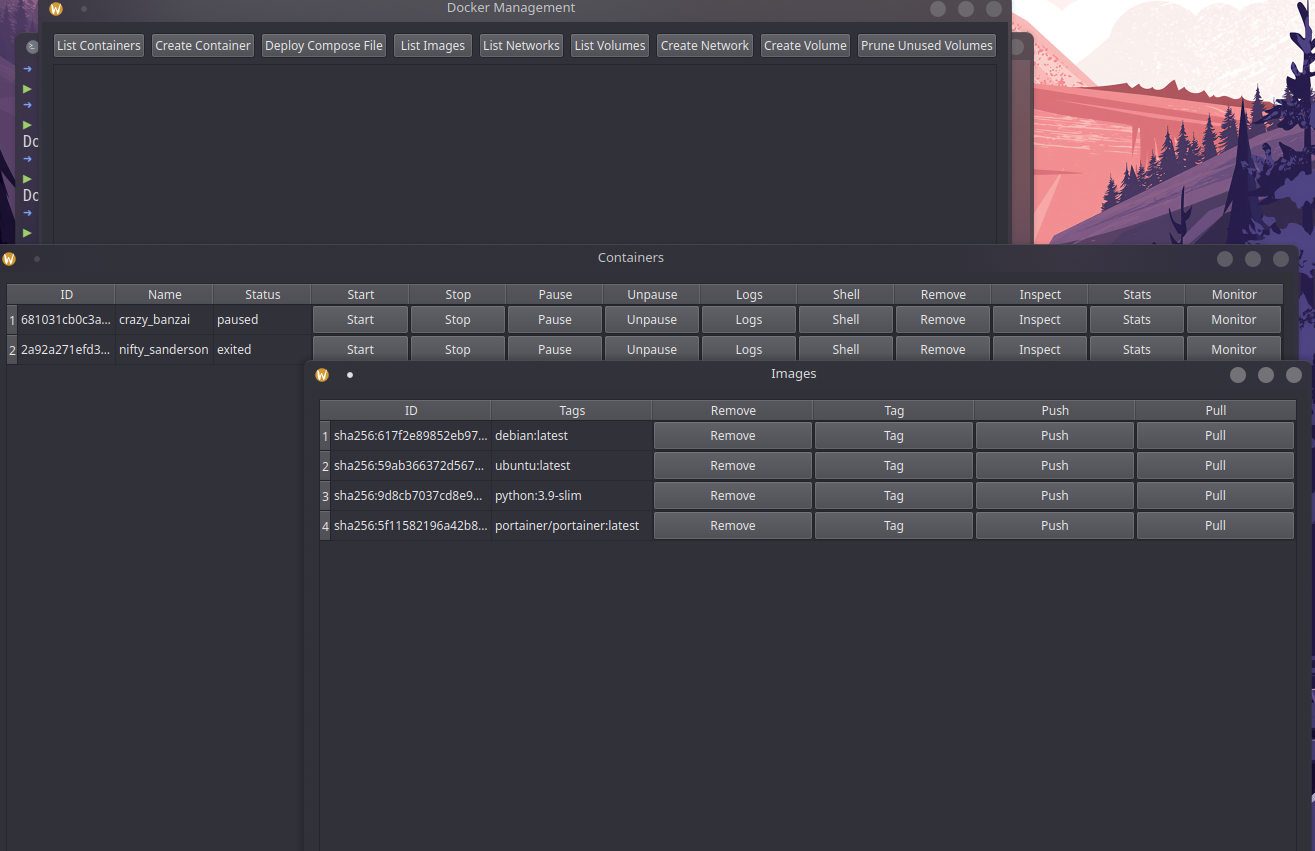
\includegraphics[width=0.7\linewidth]{images/0.4}
	\caption{Megvalósított kinézet}
	\label{fig:0.4}
\end{figure}

\subsection{Osztályok kapcsolata}
**UML DIAGRAM PLACEHOLDER**


